\chapter{Photogrammetry test flights}
\label{chap:vols-prova}

This chapter presents the two photogrammetry flights made with the complete system once the control and the GPS were stabilised (\cref{chap:proves-vol}): flight test 5, at 30~m over a park, and flight test 6, at 50~m over a field. Both ran the whole chain --~planning, automatic flight with RTK, geotagging, processing and export~-- and serve to quantify its behaviour, in particular the shutter delay (\cref{sec:retard-obturador}).

\section{Processing chain}
\label{sec:cadena-processat}

\subsection{Capture}

The mission is a \emph{grid} in Auto mode at 5~m/s with distance-based triggering. The MAP2 fires the camera by PWM and the SYNC2, on the hot shoe, returns the real instant of the exposure to the controller, which records it as a \texttt{CAM} message in the \emph{log} (the trigger command is recorded as \texttt{TRIG}). The position of each message is that of the EKF3, with RTK Fixed and GNSS \emph{yaw}.

\subsection{Photograph post-processing}
\label{sec:processament-fotos}

The photographs from the camera cannot be processed as they come out:
\begin{itemize}
    \item \textbf{Orientation.} The EXIF orientation tag of the Sony $\alpha$6000 depends on the heading (the camera points at nadir), while the pixels are always 6000~$\times$~4000. It is normalised to \emph{Orientation}=1 in a copy: only the tag changes, the pixels are not touched.
    \item \textbf{Optics.} The manual lens does not record focal length, model or aperture: they are rewritten (TTArtisan 25~mm, equivalent to 38~mm, f/5.6).
    \item \textbf{Position.} Each photograph is paired with its \emph{log} message (\texttt{CAM} or \texttt{TRIG}), the GPS tags are written into it and a geotag file is generated with the per-photo precision: 0.5~m on straight flight, 1.5~m in turns and 0.3~m vertically.
    \item \textbf{Clock.} The camera clock is off by about 9~h with respect to UTC: pairing is done by order (flight 5) or by instant (flight 6), not by the EXIF time.
\end{itemize}

The scripts that perform these steps, the flight \emph{logs}, the corrected photographs, the geotag files and the results of each processing run are archived with SHA-256 checksums, so that each result can be regenerated from the source data.

\subsection{Reconstruction}

Reconstruction is done with ODX 3.8.3 (\cref{sec:processament}). Orthophoto, DSM, point cloud and textured models are generated in EPSG:32631.

\section{Flight test 5 -- park (8 October 2026)}
\label{sec:vol5}

\subsection{Equipment and flight}

\begin{table}[H]
    \centering
    \caption{Equipment and parameters of flight test 5}
    \label{tab:vol5-equip}
    \small
    \begin{tabular}{lP{9.6cm}}
        \toprule
        Item & Value \\
        \midrule
        Controller & ArduCopter 4.6.3, Kakute H7, RC CRSF, ESC DShot300 \\
        Camera / optics & Sony $\alpha$6000 + TTArtisan 25~mm f/2, manual focus and aperture; 1/1600~s, f/5.6 \\
        Navigation & RTK Fixed for 100~\% of the flight on both receivers (GPS[0] and GPS[1]), with corrections from the own RTK base \\
        Grid & 8 passes 6.5~m apart, 7.1~m between photos (distance triggering), $\sim$30~m above the take-off point, $\sim$5~m/s \\
        Photographs & 118, between 12:26 and 12:30 (local time) \\
        Computed overlap & 75--77~\% front, 65--69~\% side; $\sim$11 images per point \\
        Camera with respect to the drone & Rotated 90$^{\circ}$ (long side along the flight direction) \\
        Hot-shoe \emph{feedback} & Not available in this flight (inverted wiring, corrected and verified afterwards on the bench) \\
        \bottomrule
    \end{tabular}
\end{table}

\subsection{Results}

Two processing runs were made with the same 118 photographs: the first with the GPS positions as they come out of the \emph{log} and the second with the positions corrected for the shutter delay (\cref{sec:retard-obturador}). The model geometry is the same; the georeferencing changes.

\begin{table}[H]
    \centering
    \caption{Processing results of flight test 5}
    \label{tab:vol5-resultats}
    \small
    \begin{tabular}{lcc}
        \toprule
        & Without correction & With delay correction \\
        \midrule
        Photos reconstructed & 118 of 118 & 118 of 118 \\
        Reprojection error & 0.90~px & 0.90~px \\
        Sparse model points & 173,084 & 173,401 \\
        Effective focal length (calibrated) & 25.72~mm & 25.74~mm \\
        Mean GSD & 0.451~cm/px & 0.452~cm/px \\
        Reconstructed area & 6,633~m\textsuperscript{2} & 6,714~m\textsuperscript{2} \\
        Dense point cloud & 38,547,923 & 38,727,582 \\
        Model--GPS difference, E / N / vert.\ (std.\ dev.) & 1.30 / 0.37 / 0.12~m & \textbf{0.40 / 0.14 / 0.11~m} \\
        CE90 / LE90 model--GPS & 1.80 / 0.19~m & \textbf{0.59 / 0.18~m} \\
        Processing time & 43~min 24~s & 41~min 34~s \\
        \bottomrule
    \end{tabular}
\end{table}

The model--GPS errors compare the model with the photo positions: they measure internal coherence, \textbf{not absolute precision}, which requires independent check points (\cref{sec:gcp}). The delay correction reduces the horizontal difference from the order of 1.3~m to $\sim$0.4~m, and the georeferenced camera positions move at most 0.31~m between the two runs, with a model rotation of $0.2^{\circ}$.

\begin{figure}[H]
    \centering
    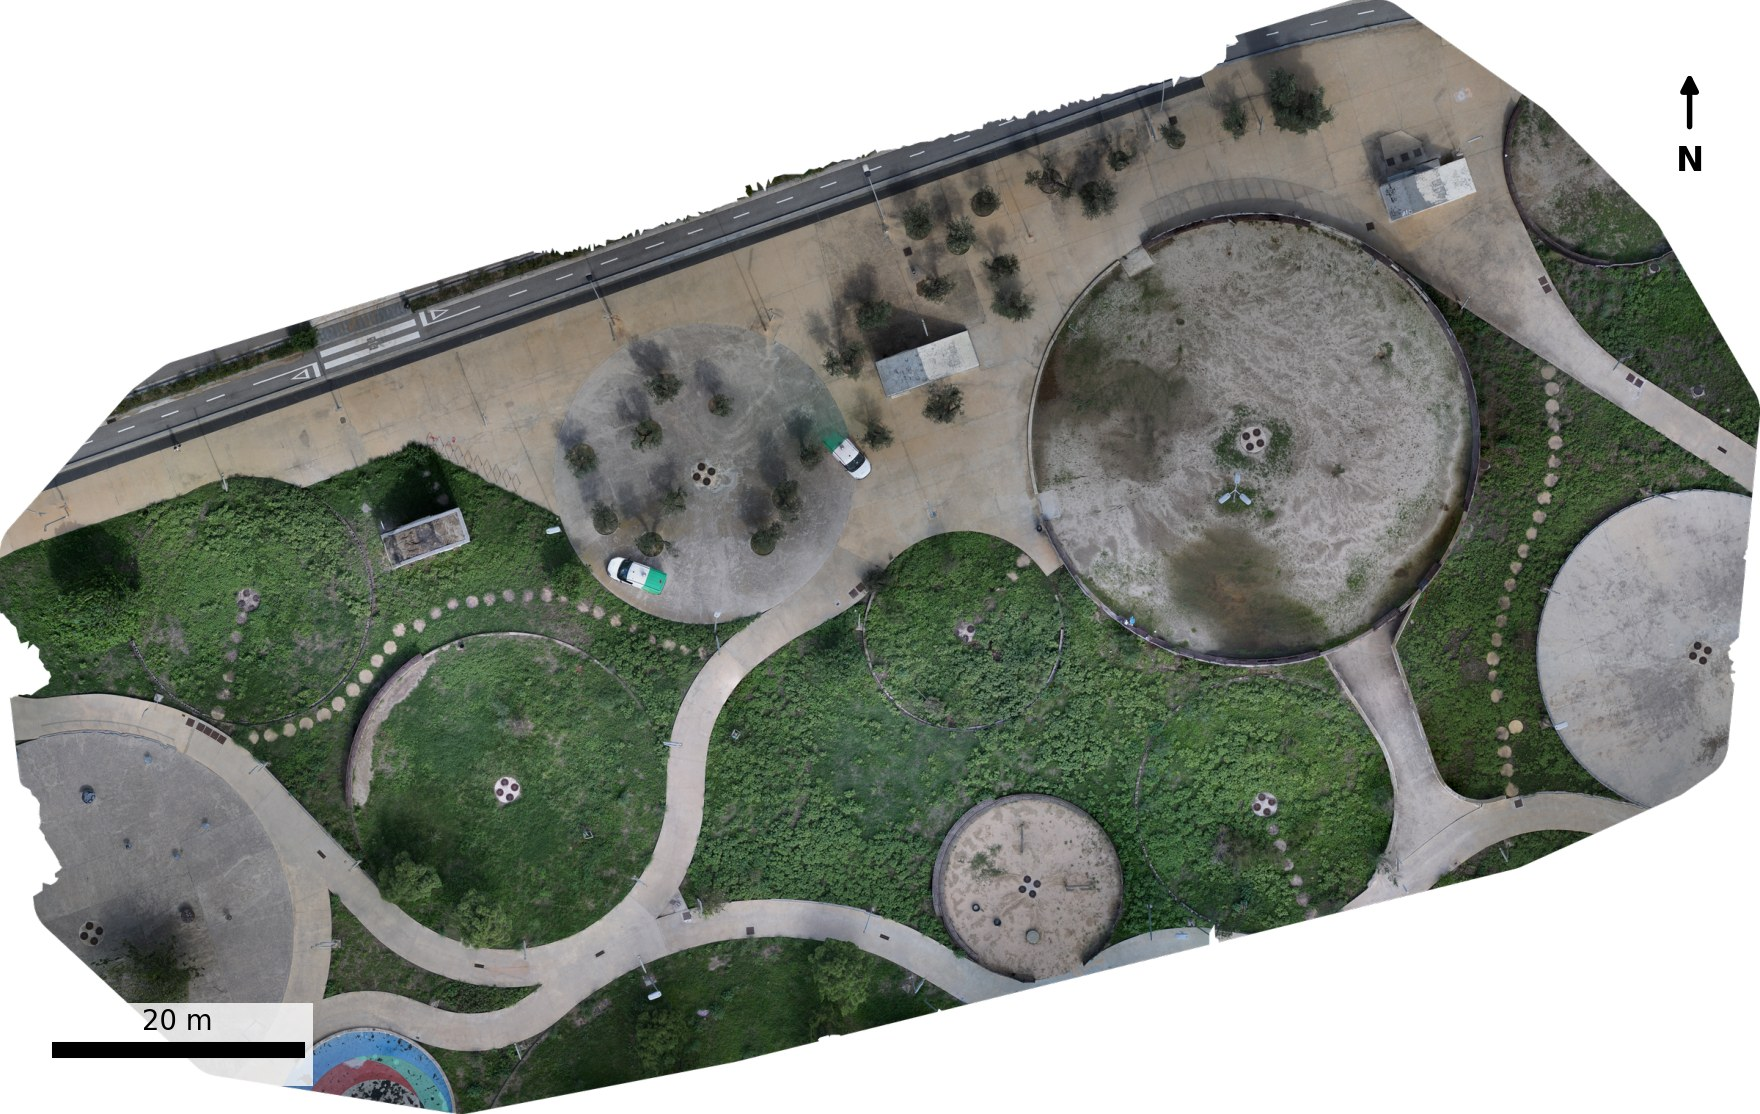
\includegraphics[width=\textwidth]{img/vol5_ortofoto.jpg}
    \caption{Orthophoto of flight test 5 (1~cm/px, EPSG:32631), processed with positions corrected for the shutter delay.}
    \label{fig:vol5-ortofoto}
\end{figure}

The orthophoto (14,084~$\times$~8,918~px at 1~cm/px) is coherent: no seams or bowl-shaped deformation, with consistent paths and roundabouts and sharp at 1:1 scale (concrete joints, individual leaves). The DSM (7,041~$\times$~4,458~px at 2~cm/px) is clean in the interior (flat buildings, trees as relief); the first and last pass and the edges show streaks because of few views, so it is advisable to crop the DSM to the polygon of interest or to extend the flight plan one \emph{footprint} beyond the area.

\begin{figure}[H]
    \centering
    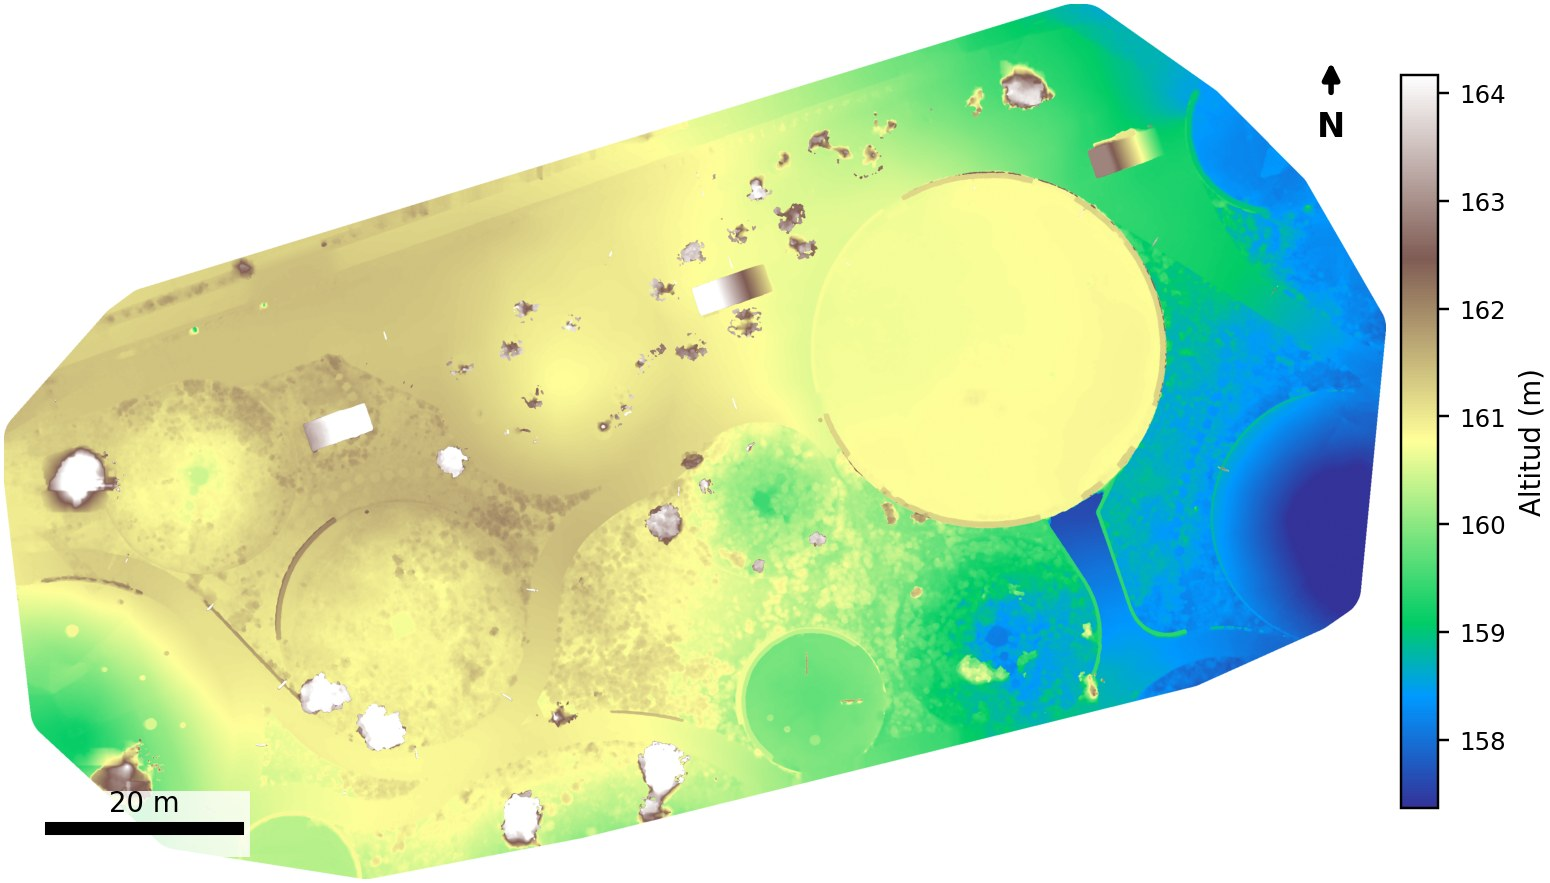
\includegraphics[width=\textwidth]{img/vol5_dsm.jpg}
    \caption{Digital surface model of flight test 5 (2~cm/px). The white gaps are treetops above the palette range.}
    \label{fig:vol5-dsm}
\end{figure}

\section{Flight test 6 -- field (13 October 2026)}
\label{sec:vol6}

\subsection{Equipment and flights}

Flight test 6 consists of two flights at $\sim$50~m (area of $\sim$180~$\times$~150~m) with the same drone and camera as 5 and with the battery parameters already calibrated. The hot-shoe \emph{feedback} (\texttt{CAM}) and the planning at 50~m were validated. They were made at dawn, with the sun between $-3^{\circ}$ and $+1^{\circ}$ above the horizon, so the photographs came out very dark.

\begin{table}[H]
    \centering
    \caption{Log of the two flights of flight test 6}
    \label{tab:vol6-logs}
    \small
    \begin{tabular}{lcc}
        \toprule
        & Flight 1 (07:46) & Flight 2 (07:57) \\
        \midrule
        mAh consumed (\texttt{CurrTot} / integral) & 2,326 / 2,306 & 2,434 / 2,426 \\
        Motors running & 5.5~min & 11.3~min (two arms) \\
        Voltage initial / minimum / final & 24.65 / 21.25 / 21.95~V & 24.73 / 21.13 / 21.95~V \\
        Current average / maximum & 25 / 56~A & 22 / 58~A \\
        Low-battery \emph{failsafe} & 268~s, 21.52~V, 1,887~mAh & 635~s, 21.48~V, 2,012~mAh \\
        Triggers \texttt{TRIG} / \texttt{CAM} / photos & 94 / 93 / 94 & 110 / 110 / 110 \\
        \bottomrule
    \end{tabular}
\end{table}

\begin{itemize}
    \item \textbf{Battery.} Both flights end by low-battery \emph{failsafe} when only 47--50~\% of the 4,000~mAh has been used: the instantaneous voltage drops below 21.6~V under load (\texttt{BATT\_FS\_VOLTSRC=0}). The mAh must be compared with what the charger returns.
    \item \textbf{Exposure.} 1/1600~s, f/5.6, ISO 1600 (ceiling of the automatic ISO): the photographs are about 6~\emph{stops} underexposed, and the scene light is 8.5--11.9~\emph{stops} below that of flight 5 (sun at 40$^{\circ}$). The maximum margin of the camera is 5.7~\emph{stops}. It is not a fault: it is a light limitation.
    \item \textbf{Feedback.} With \texttt{TRIG}, \texttt{CAM} and photographs in a 1:1 ratio (110 of 110 in flight 2), pairing is done by instant. There is one manual photo without \texttt{TRIG} and one \texttt{TRIG} without a photo.
\end{itemize}

\pendent{Repeat this flight with the sun more than 10--15$^{\circ}$ high, which is the condition that makes it usable (the current batch only serves as a test).}

\subsection{Processing of flight 2}

Flight 1 is not usable (the digital gain $\times 551$ does not recover signal: 2 matches between consecutive photos, the same as the noise). From flight 2 the 110 photographs were processed with a linear gain of $\times 2$ to $\times 97$ (median $\times 49$); \textbf{the geometry is valid, but the colours and radiometric values are not} (blue-green tint, high noise), so this batch is not suitable for colour or vegetation indices.

\begin{table}[H]
    \centering
    \caption{Processing results of flight 2 of flight test 6}
    \label{tab:vol6-resultats}
    \begin{tabular}{ll}
        \toprule
        Item & Value \\
        \midrule
        Photos reconstructed & 110 of 110 (1 component) \\
        Sparse model points / observations & 101,094 / 354,361 \\
        Reprojection error & 1.82~px \\
        Mean GSD / reconstructed area & 0.743~cm/px / 30,626~m\textsuperscript{2} \\
        Dense point cloud & 27,207,845 points \\
        Camera calibration & focal length 25.79~mm \\
        Model--GPS difference (E / N / vert.) & 0.30 / 0.32 / 0.30~m; CE90 0.57~m, LE90 0.27~m \\
        Orthophoto / DSM resolution & 3~cm/px / 5~cm/px \\
        Processing time & 29~min 42~s \\
        \bottomrule
    \end{tabular}
\end{table}

The quality is lower than in flight 5 (reprojection of 1.82~px versus 0.90~px): this is consistent with the noise of the images, which makes a larger working resolution (3~cm/px) preferable. The orthophoto (7,799~$\times$~7,071~px) shows the field, the paths, the bend of the path and a white vehicle recognisably, with a blue-green tint and noise visible and an irregular western edge. The DSM (4,679~$\times$~4,242~px) is detailed in the interior (furrows, ruts) and has streaks and an interpolation grid at the western and north-western edge.

\begin{figure}[H]
    \centering
    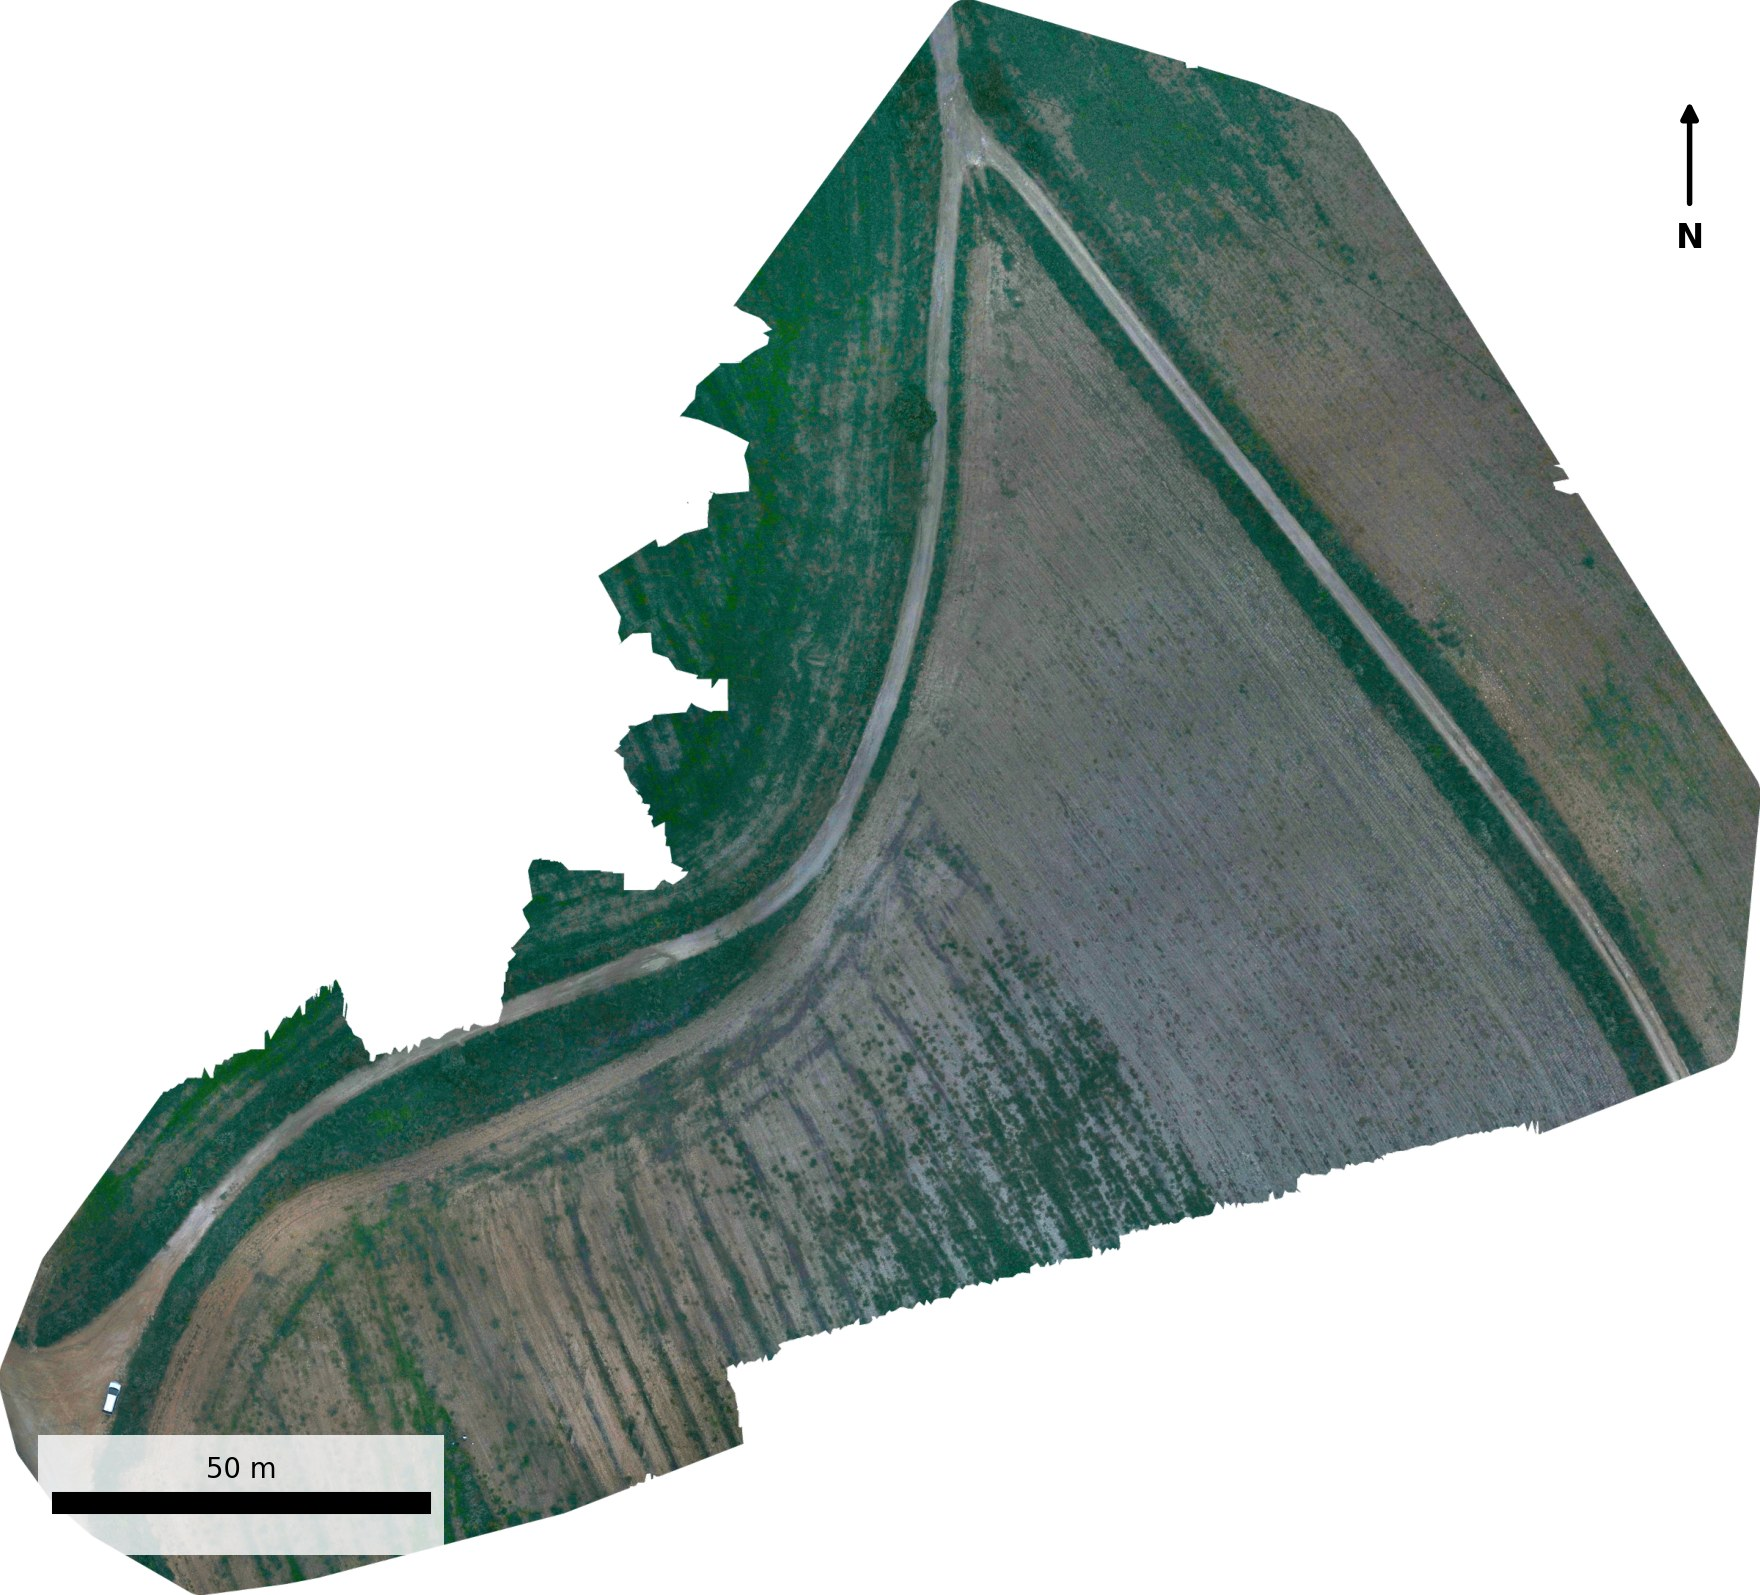
\includegraphics[width=0.85\textwidth]{img/vol6_ortofoto.jpg}
    \caption{Orthophoto of flight 2 of test 6 (3~cm/px). The images were digitally enhanced: only the geometry is valid, not the colour.}
    \label{fig:vol6-ortofoto}
\end{figure}

\begin{figure}[H]
    \centering
    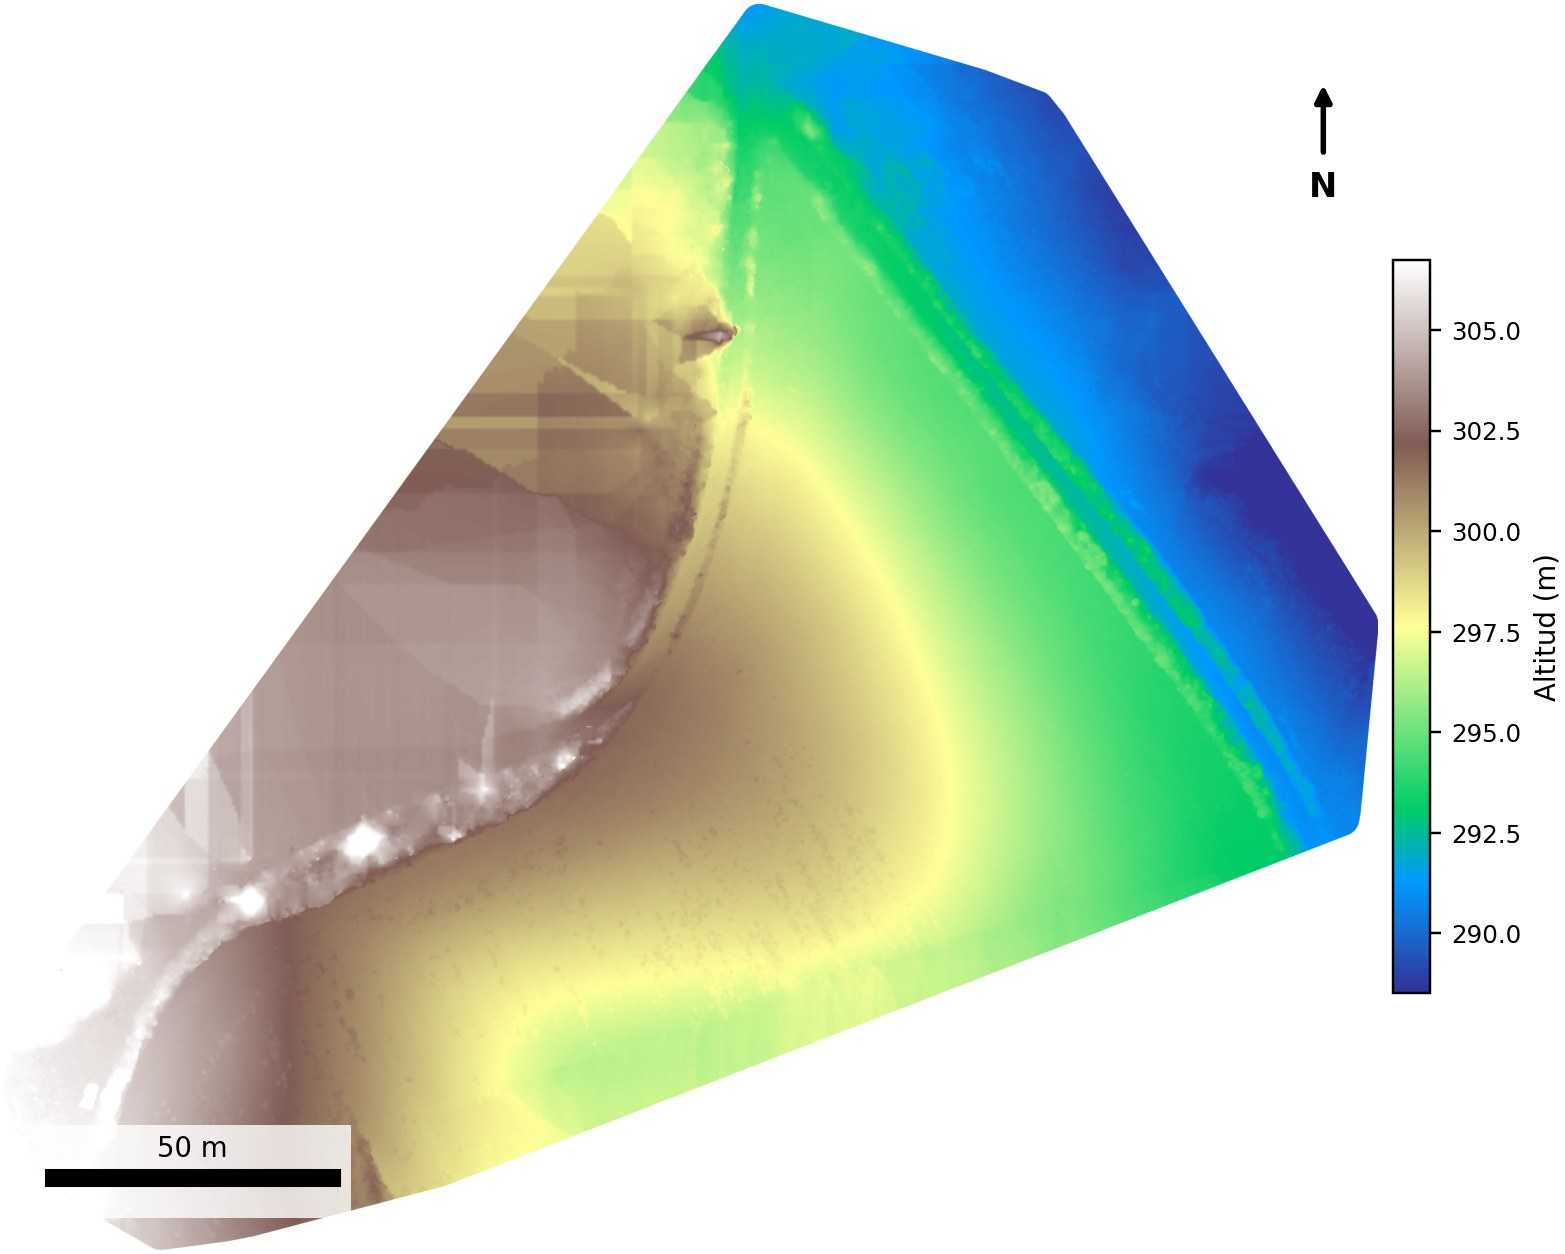
\includegraphics[width=0.85\textwidth]{img/vol6_dsm.jpg}
    \caption{Digital surface model of flight 2 of test 6 (5~cm/px).}
    \label{fig:vol6-dsm}
\end{figure}

\section{Shutter delay}
\label{sec:retard-obturador}

The trigger command of the controller and the real exposure do not coincide: between them lies the delay of the MAP2, of the camera and, possibly, of the GPS/EKF position. Since the drone moves at $\sim$5~m/s, a delay of 0.27~s equals $\sim$1.3~m of displacement, far above the centimetre-level precision sought.

\subsection{Method}

For each photo, the GPS position from the \emph{log} is compared with the camera position reconstructed by the photogrammetric model. If the delay is $\tau$, the GPS $-$ model residual is $-v\tau$: it has the opposite sign on the outbound and return passes and a global offset close to zero, which distinguishes it from a systematic georeferencing error.

\subsection{Results}

\begin{table}[H]
    \centering
    \caption{Estimates of the shutter delay}
    \label{tab:retard}
    \small
    \begin{tabular}{P{5.2cm}P{4.2cm}P{4.6cm}}
        \toprule
        Measurement & Delay & Notes \\
        \midrule
        Flight 5, \texttt{TRIG} positions & $\tau = 0.268 \pm 0.009$~s & ENE 0.277~$\pm$~0.007; WSW 0.267~$\pm$~0.014 \\
        Flight 5 with corrected positions & residual $0.004 \pm 0.007$~s & Horizontal residual median 1.38~m $\rightarrow$ 0.35--0.49~m \\
        Flight 6, \texttt{TRIG}$\rightarrow$\texttt{CAM} & median 0.34~s (0.11--0.40) & Measured directly in the \emph{log} \\
        Flight 6, \texttt{CAM} positions & residual $-0.056 \pm 0.011$~s & The \texttt{CAM} position is $\sim$56~ms ahead of the exposure \\
        Flight 6, \texttt{TRIG}$\rightarrow$exposure & $0.34 - 0.056 \approx 0.28$~s & Agrees with flight 5 by an independent route \\
        Bench, command$\rightarrow$shutter & 0.12--0.19~s & Does not explain all the delay in flight \\
        \bottomrule
    \end{tabular}
\end{table}

Two independent methods --~the photogrammetric residual of flight 5 and the combination of \texttt{TRIG}, \texttt{CAM} and residual of flight 6~-- agree on 0.27--0.28~s. It is an \emph{effective} delay: it adds up that of the shutter and, possibly, that of the GPS/EKF position, and a fixed forward offset of the antenna with respect to the camera is confounded with it (if left as an unknown, the delay comes out at 0.34~$\pm$~0.03~s and the offset at 0.32~$\pm$~0.16~m, and they cannot be separated). The bench delay does not explain the whole in-flight value; it cannot be separated without \emph{feedback}.

\subsection{Consequences for geotagging}

With \emph{feedback} (\texttt{CAM}), the position is that of the real exposure and only a residual delay of $-0.056$~s remains ($\sim$0.3~m at 5~m/s), which can be compensated. Without \emph{feedback} the position must be shifted by $v\cdot\tau$ with $\tau \approx 0.27$~s and wider per-photo precisions. This is the reason why the hot-shoe \emph{feedback} is mandatory for centimetre-level precision (\cref{sec:decisions}).

\section{Balance of the test flights}
\label{sec:balanc-vols}

\textbf{What has worked.}
\begin{itemize}
    \item The complete chain, from planning to the DSM, with RTK Fixed throughout the flight on both receivers and valid GNSS \emph{yaw}.
    \item A geometry of photogrammetric quality: reprojection of 0.90~px, 118 of 118 photos reconstructed and a GSD (0.451~cm/px) consistent with the flight height and the calibrated focal length (\cref{sec:planificacio-vol}).
    \item The hot-shoe \emph{feedback} (110 of 110 in flight 6) and the independent quantification of the shutter delay.
\end{itemize}

\textbf{Limitations.}
\begin{itemize}
    \item There are no control or check points: an absolute precision cannot be stated. The model--GPS figures are internal coherence.
    \item The absolute position depends on the RTK base, which in these flights ran a \emph{survey-in} in every session with the antenna at 122~cm (\cref{subsec:muntatge-base}). The resulting position was not recorded, and the absolute error is of the order of metres, common to the whole flight.
    \item For flight 5 the weather conditions, the in-flight mass and the battery used are not available: the \emph{log} and the photographs are the only record.
    \item Light limits the operation: flights must be made with the sun more than 10--15$^{\circ}$ high (or, with little light, 1/800~s, f/4 and ISO 3200 at the limit).
    \item Endurance is short: the low-battery \emph{failsafes} act at half consumption because of the voltage drop under load (\cref{sec:autonomia}).
    \item The DSM shows streaks at the periphery: the flight plan must be extended one \emph{footprint} beyond the area of interest.
\end{itemize}

\textbf{Next steps.} Repeat the field flight with the sun high, measure ground control and check points to establish absolute precision, re-estimate the delay with \emph{feedback} and improve endurance (\cref{sec:propulsor}). The complete list of pending tasks is in \cref{sec:pendents-proves-vol}.

\pendent{The absolute precision (horizontal and vertical) of the final product remains unmeasured: all the errors in this chapter are internal coherence.}
